\documentclass[aps,prd,twocolumn,superscriptaddress,nofootinbib,floatfix]{revtex4-2}

\usepackage{amsmath,amssymb}
\usepackage{graphicx}
\usepackage{booktabs}
\usepackage{xcolor}
\usepackage[colorlinks=true,linkcolor=blue!50!black,citecolor=blue!50!black,urlcolor=blue!50!black]{hyperref}

% Values that exist only on the analysis server and must be filled in before submission.
\newcommand{\TBD}[1]{\textcolor{red}{[#1]}}
\newcommand{\pfa}{p_{\rm FA}}
\newcommand{\eff}{\varepsilon}
\newcommand{\msun}{M_\odot}
\newcommand{\PIR}{PI-ResNet}

\begin{document}

\title{Recognising the two images of a strongly lensed gravitational wave:\\
a time-domain pair test, its calibrated performance for the Einstein Telescope,\\
and what the GWTC-3, O4a and O4b catalogues demand of it}

\author{\TBD{Author list and affiliations}}

\date{\today}

\begin{abstract}
A galaxy lying close to the line of sight can split the gravitational wave from one binary black-hole merger into two or more copies that reach the Earth hours to months apart.
The copies share the same intrinsic waveform and the same sky position, but differ in arrival time, in amplitude, and, for some images, by a fixed phase shift.
Recognising such pairs among hundreds (today) or hundreds of thousands (with the Einstein Telescope) of unrelated mergers is a needle-in-a-haystack problem.
We study \PIR{}, a residual neural network that reads the two recorded strain segments directly and returns a single number measuring how likely they are to be copies of one signal.
Using simulated Einstein Telescope data in stationary Gaussian noise, we fix the acceptance threshold in advance from a large set of deliberately unrelated event pairs, exactly as the background is estimated in gravitational-wave searches, and only then measure performance on an independently generated catalogue.
When the threshold is set so that only one unrelated pair in a thousand is accepted, \PIR{} recovers $54\%$ of lensed pairs produced by galaxy-like lenses (singular isothermal spheres) and $23\%$ of those produced by compact point-mass lenses, compared with $38\%$ and $9\%$ for a baseline that, following earlier work, first converts each signal into a time--frequency image.
Recovery is limited mainly by the loudness of the fainter image.
We then place these numbers in the context of the real LIGO--Virgo--KAGRA catalogues.
The 168 binary black holes we use from O1--O3 (GWTC-2.1/GWTC-3) and O4b (GWTC-5.0) already form $14\,028$ possible pairs, while only ${\sim}0.2$ genuine lensed pairs are expected.
Requiring a physically allowed time delay, a common sky position and a common detector-frame chirp mass removes $95\%$ of these pairs while keeping $98\%$ of simulated lensed pairs, but $637$ pairs survive; a pair test applied to them must accept fewer than about $1.6\times10^{-4}$ of unrelated pairs to keep the expected number of false claims below $0.1$.
This sets a concrete target for the next generation of pair tests, which must operate on real detector noise and include the O4a data (GWTC-4.0).
\end{abstract}

\maketitle

%=====================================================================
\section{Introduction}
\label{sec:intro}
%=====================================================================

Gravitational lensing by intervening matter deflects gravitational waves in the same way as it deflects light~\cite{SchneiderEhlersFalco,NarayanBartelmann,Wang1996,Nakamura1998,TakahashiNakamura2003}.
When a compact binary lies almost directly behind a massive galaxy, more than one path connects source and observer and the detectors record several copies, or \emph{images}, of the same merger.
Because the wavelength of a ground-based gravitational-wave signal ($\sim 10^3$\,km) is tiny compared with the size of a galaxy, the images are described by geometric optics: each is a rescaled, time-shifted and, in some cases, phase-shifted copy of the unlensed signal~\cite{DaiVenumadhav2017,Ezquiaga2021}.
For galaxy-scale lenses the copies arrive minutes to months apart~\cite{Haris2018,Oguri2018}, so that a lensed merger appears in a catalogue as two apparently independent events.

Finding such repeated events would be scientifically valuable.
It would test the propagation of gravitational waves over cosmological distances, constrain the population of lens galaxies and of the merging binaries~\cite{Xu2022}, and could localise a merger to sub-arcsecond precision by identifying its lensed host galaxy~\cite{Hannuksela2020loc}.
The expected rate is, however, small: of order one detected binary black hole in a thousand should have a detectable lensed counterpart at the sensitivity of current detectors~\cite{Ng2018,Li2018,Oguri2018,Wierda2021,Xu2022}.
Searches through the first three observing runs (O1--O3) found no convincing lensed pair~\cite{Hannuksela2019,LiuO2,LVKO3a,LVKO3,Janquart2023followup}, while individual candidates such as GW170104--GW170814~\cite{Dai2020} illustrated how difficult it is to separate a genuine lensed pair from a chance resemblance.

The difficulty is combinatorial.
A catalogue of $N$ events contains $N(N-1)/2$ possible pairs.
The fourth observing run (O4) has more than doubled the number of confident binary black holes~\cite{GWTC4,GWTC5}, and the Einstein Telescope (ET)~\cite{Punturo2010,Maggiore2020,Branchesi2023} is expected to detect of order $10^5$ binary black holes per year, i.e.\ $\sim 5\times10^{9}$ pairs per year.
Every pair test therefore faces the same question as any search for a rare signal: how often does it accept a pair that is \emph{not} lensed, and how many genuine pairs does it recover at that acceptance rate?
Rigorous Bayesian tests that compare full parameter estimates of the two events~\cite{Haris2018,LoHernandez2023,Janquart2021GOLUM} answer this question well but are too expensive to apply to every pair; machine-learning tests~\cite{Goyal2021,SEMD} are fast, but their acceptance rates have often been quoted at a single, uncalibrated threshold.

In this paper we study a fast pair test, \PIR{}, that compares the two recorded strain time series directly.
Our aims are (i) to measure its performance in the way a gravitational-wave physicist would measure the performance of a search, with the background rate fixed in advance and the efficiency measured on independent data; (ii) to understand which physical properties of a lensed pair make it easy or hard to recognise; and (iii) to ask what the real catalogues---GWTC-2.1/GWTC-3 for O1--O3~\cite{GWTC21,GWTC3}, GWTC-4.0 for O4a~\cite{GWTC4} and GWTC-5.0 for O4b~\cite{GWTC5}---require of such a test before it could support a discovery claim.

\paragraph*{Results in brief.}
In simulated Einstein Telescope data, when the threshold is set to accept one unrelated pair in a thousand, \PIR{} recovers $54\%$ of galaxy-lensed pairs and $23\%$ of point-mass-lensed pairs, about $15$ percentage points more than a time--frequency-image baseline (Sec.~\ref{sec:results}).
The recovered fraction is controlled mainly by the signal-to-noise ratio (SNR) of the fainter image.
The test is insensitive to the time delay by construction and, in a controlled experiment, also to the phase shift of type-II images (Sec.~\ref{sec:diagnostics}).
In the real catalogues, simple physical requirements reduce $14\,028$ pairs to $637$, but even at the strictest threshold we calibrated, a pair test alone would still produce false claims at a rate comparable to the expected number of genuine lensed pairs (Sec.~\ref{sec:catalogue}).
A pair test is therefore best used as one fast stage between a physical pre-selection and a full Bayesian follow-up.

%=====================================================================
\section{What lensing changes, and what it leaves unchanged}
\label{sec:physics}
%=====================================================================

\subsection{Images in geometric optics}

Let $\tilde h(f)$ be the frequency-domain strain that an observer would record without the lens.
Image $j$ is then~\cite{DaiVenumadhav2017,Ezquiaga2021}
\begin{equation}
\tilde h_j(f) = \sqrt{|\mu_j|}\; \exp\!\left[-i\pi n_j\,{\rm sgn}(f)\right]\; e^{2\pi i f t_j}\;\tilde h(f),
\label{eq:image}
\end{equation}
where $\mu_j$ is the magnification, $t_j$ the arrival time, and $n_j=0,\tfrac12,1$ the Morse index for an image formed at a minimum, saddle point, or maximum of the light-travel time (type I, II and III images).
A type-II image is therefore the Hilbert transform of the unlensed waveform, i.e.\ every frequency component is shifted in phase by $\pi/2$ (Fig.~\ref{fig:schematic}).
Equation~\eqref{eq:image} immediately tells us what a pair test may and may not use:
\begin{itemize}
\item \emph{Unchanged:} the detector-frame masses and spins, hence the frequency evolution (the ``chirp'') of the waveform; the sky position, because image separations of order an arcsecond are far below gravitational-wave localisation accuracy; the orbital inclination and polarisation angle.
\item \emph{Changed:} the arrival time; the amplitude, by $\sqrt{|\mu_j|}$, so that the luminosity distance inferred from each image is biased to $D_L/\sqrt{|\mu_j|}$; and, for type-II images, the waveform phase.
\end{itemize}
In addition, because the Earth rotates between the two arrivals, the detector views the source with a different orientation, which changes the recorded amplitude and phase of each image independently of the lens.
A pair test must therefore judge the \emph{shape} of the two waveforms rather than their absolute amplitude.

\begin{figure}[t]
\centering
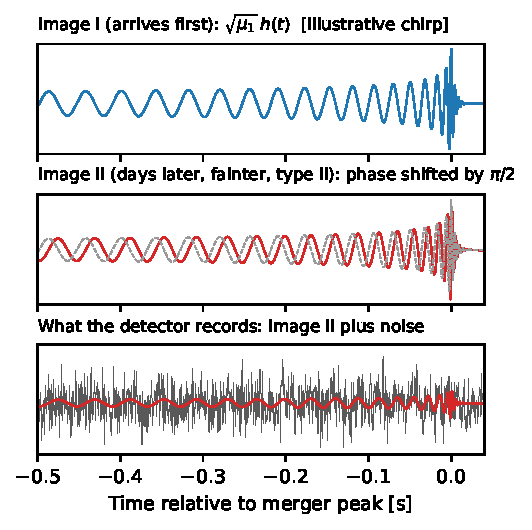
\includegraphics[width=\columnwidth]{figures/fig_lensing_schematic.pdf}
\caption{What a pair test must recognise.
Top: the first, brighter (type-I) image of an illustrative chirp.
Middle: the second, fainter image of a type-II (saddle-point) image; the dashed grey curve shows the same signal without the $\pi/2$ Morse phase shift of Eq.~\eqref{eq:image}.
Bottom: the second image as it would appear in detector noise.
\PIR{} receives the two noisy segments, each normalised to unit variance, and must decide whether they are copies of one signal.}
\label{fig:schematic}
\end{figure}

\subsection{Two lens models}

We consider two idealised lenses that bracket the physical situations of interest.
For both, the source position is described by the dimensionless impact parameter $y$, the angular offset of the source from the lens centre in units of the Einstein radius; two images form for $y<1$ (singular isothermal sphere) or any $y$ (point mass), and smaller $y$ means a more nearly aligned, more strongly magnified system.

\emph{Singular isothermal sphere (SIS).}
A simple model of the dark-matter halo of a galaxy, characterised by its velocity dispersion $\sigma_v$.
The two images have $\mu_\pm = 1\pm 1/y$ and arrive with a delay~\cite{NarayanBartelmann}
\begin{equation}
\Delta t_{\rm SIS} = \frac{32\pi^2}{c}\left(\frac{\sigma_v}{c}\right)^{4}(1+z_l)\,\frac{D_l D_{ls}}{D_s}\,y,
\label{eq:sis}
\end{equation}
where $z_l$ is the lens redshift and $D_l$, $D_s$, $D_{ls}$ are angular-diameter distances to the lens, to the source, and from lens to source.

\emph{Point mass (PM).}
A compact lens of mass $M_l$, for which $\mu_\pm = \tfrac12 \pm (y^2+2)/(2y\sqrt{y^2+4})$ and
\begin{equation}
\Delta t_{\rm PM} = \frac{4GM_l(1+z_l)}{c^3}\left[\frac{y\sqrt{y^2+4}}{2} + \ln\frac{\sqrt{y^2+4}+y}{\sqrt{y^2+4}-y}\right].
\label{eq:pm}
\end{equation}
In both models the second image is a type-II (saddle-point) image.
For $y\le 0.3$, the range simulated here, the ratio of the two magnifications lies between $1$ and about $1.9$.

%=====================================================================
\section{Simulated Einstein Telescope catalogues}
\label{sec:sims}
%=====================================================================

We simulate binary black-hole mergers with source-frame component masses drawn uniformly between $10$ and $100\,\msun$, isotropically oriented precessing spins with magnitudes up to $0.99$, isotropic sky positions and orientations, and redshifts between $0.01$ and $1$ distributed uniformly in comoving volume in a Planck 2018 cosmology~\cite{Planck2018}.
Waveforms are computed with the precessing, higher-harmonic model IMRPhenomXPHM~\cite{XPHM} using \textsc{bilby}~\cite{bilby}, from $20$\,Hz, and projected onto the three interferometers of the triangular Einstein Telescope with stationary Gaussian noise of the \TBD{ET-D} design sensitivity.
For lensing we use \textsc{lenstronomy}~\cite{lenstronomy}.
Each source is lensed with $y$ drawn uniformly in $[0.01,0.3]$ and the lens placed at $z_l=z_s/2$.
SIS lenses have $\sigma_v$ uniform in $[100,500]\,{\rm km\,s^{-1}}$; point-mass lenses have $M_l$ uniform in $[10^{8},10^{10}]\,\msun$.
The resulting delays (Fig.~\ref{fig:delays}, blue and red) have medians of $26$ days (SIS) and $0.4$ days (PM).

\paragraph*{Two independent catalogues.}
We generate two catalogues from the same distributions but with independent random draws of sources, lenses and noise.
Catalogue~A (2\,500 lensed sources for each lens model, plus 5\,000 unlensed events) is used only to train the networks and to choose when to stop training.
Catalogue~B, of the same size, is used only to set acceptance thresholds and to measure performance.
We verified, by comparing file checksums, source parameters and waveform samples, that no source or noise realisation appears in both.
Catalogue~B is an independent \emph{realisation} of the same simulated Universe; it is not a test against a different astrophysical population or against real detector noise.

\paragraph*{What counts as a pair.}
A \emph{lensed pair} consists of the two images of one source.
To estimate how often unrelated events are accepted we build \emph{unrelated pairs} of two kinds: $70\%$ pair the first image of one lensed source with the second image of a different lensed source (the most realistic and most difficult background, since both events are genuine lensed images processed in exactly the same way), and $30\%$ pair a lensed image with an unlensed event.

\paragraph*{What the network sees.}
Each event is represented by the final \TBD{2\,s} of its detector strain, aligned on the peak of the signal and resampled to \TBD{2\,048\,Hz}.
Each segment is shifted to zero mean, scaled to unit variance, and multiplied by $\pm1$ so that its largest excursion is positive.
These steps remove the absolute amplitude (and therefore the magnification) and an overall sign, so that the comparison relies on the waveform shape.
Peak alignment also removes the arrival time; the consequences are discussed in Sec.~\ref{sec:diagnostics}.

%=====================================================================
\section{The pair test and how its threshold is set}
\label{sec:method}
%=====================================================================

\subsection{PI-ResNet}

\PIR{} applies the same one-dimensional convolutional network to each of the two segments and then compares the results (Appendix~\ref{app:architecture}).
The network is built from residual blocks~\cite{ResNet}, in which each block learns a correction to its input; this design allows deep networks to be trained stably.
The ``PI'' refers to physics-inspired design choices rather than to the imposition of lensing equations:
(i) a periodic activation function~\cite{Snake} suited to oscillatory signals such as a chirp;
(ii) channel re-weighting~\cite{SENet}, which lets the network emphasise the frequency-like features that carry most information; and
(iii) a symmetric comparison of the two summaries---their element-wise product and absolute difference---so that the answer does not depend on which event is called ``first''.
The output is a number between $0$ and $1$, which we call the \emph{pair score}.
A high score means that the two segments look like copies of one signal.
The network was trained for $300$ passes through catalogue~A with the learning settings listed in Appendix~\ref{app:architecture}.

\subsection{A time--frequency baseline}

For comparison we train a baseline that follows the SEMD approach~\cite{SEMD}: each segment is first converted into a constant-$Q$ time--frequency map~\cite{BrownCQT}, i.e.\ an image of how the signal power is distributed in time and frequency, and the two images are then compared by a vision-transformer network~\cite{DeiT}.
We call it CQT--DeiT.
It is trained on exactly the same events and evaluated on exactly the same pairs as \PIR{}.

\subsection{Setting the threshold from the background}
\label{sec:threshold}

A pair test is only useful if we know how often it accepts unrelated pairs.
We therefore follow the logic of gravitational-wave searches, where the background is estimated by time-shifting the data of different detectors to create many signal-free coincidences~\cite{GW150914search}.
Here we construct $100\,000$ unrelated pairs from a \emph{threshold-setting} subset ($30\%$ of the sources of catalogue~B), compute their scores, and choose the threshold so that a fraction $\pfa$ of them exceeds it.
We call $\pfa$ the \emph{false-alarm probability per pair}.
We use three values: $\pfa=10^{-2}$, $10^{-3}$ (our primary choice) and $10^{-4}$.
With $100\,000$ background pairs, the strictest threshold is set by only ten background pairs, so its position is uncertain at the ${\sim}30\%$ level (Poisson statistics); we therefore regard $10^{-4}$ as a diagnostic of the extreme tail rather than as a headline result.

The thresholds, together with every other analysis choice, were frozen before any score from the remaining $70\%$ of catalogue~B---the \emph{measurement} subset---was examined.
This is the equivalent of a blind analysis.
In the measurement subset we record, for each threshold, the \emph{detection efficiency} $\eff$, i.e.\ the fraction of genuine lensed pairs whose score exceeds the threshold, and we check that the fraction of a fresh set of $100\,000$ unrelated pairs above threshold is consistent with the target $\pfa$.

\subsection{How the uncertainties are obtained}

Lensed and unrelated pairs built from the same source are not statistically independent.
We therefore divide the sources into ten groups, repeatedly draw groups at random with replacement, recompute every quantity, and quote the range containing the central $95\%$ of the $10\,000$ repetitions~\cite{Efron1979}.
When we compare \PIR{} with CQT--DeiT we apply both to the identical pairs in each repetition and quote the range of the \emph{difference}, so that fluctuations common to both methods cancel.
Further statistical details, including summary numbers that are customary in the machine-learning literature, are collected in Appendix~\ref{app:stats}.

%=====================================================================
\section{Performance on the simulated catalogue}
\label{sec:results}
%=====================================================================

\subsection{Detection efficiency at a fixed false-alarm probability}

Figure~\ref{fig:eff} and Table~\ref{tab:main} summarise the main result.
At $\pfa=10^{-3}$, \PIR{} recovers $\eff=0.535$ ($0.510$--$0.563$) of SIS-lensed pairs and $0.227$ ($0.211$--$0.246$) of point-mass-lensed pairs.
CQT--DeiT recovers $0.377$ and $0.093$.
The gains, $0.158$ ($0.137$--$0.181$) and $0.135$ ($0.117$--$0.151$), are many times larger than their uncertainties.
Working directly with the time series therefore extracts more of the information that distinguishes a genuine lensed pair from a chance resemblance than first converting each signal into a time--frequency image.

The advantage does not hold uniformly in the far tail.
At $\pfa=10^{-4}$, \PIR{} recovers \emph{fewer} SIS-lensed pairs than CQT--DeiT (difference $-0.040$, range $-0.061$ to $-0.017$), and for point-mass lenses the two are indistinguishable (difference $+0.009$, range $-0.002$ to $+0.021$).
We checked that this is not an artefact of how the scores are numerically squashed into $[0,1]$: recomputing the thresholds on the unsquashed network output selects exactly the same pairs.
Because the $10^{-4}$ threshold rests on only ten background pairs (Sec.~\ref{sec:threshold}), establishing which method is better there requires a much larger background set.

\begin{figure}[t]
\centering
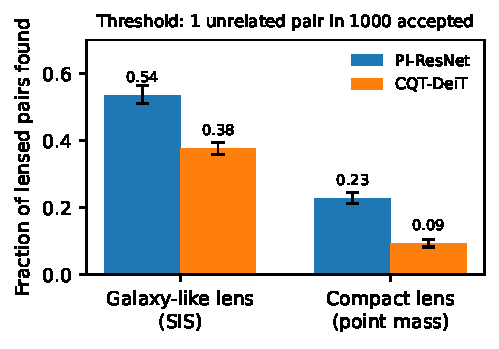
\includegraphics[width=0.95\columnwidth]{figures/fig_efficiency_1e-3.pdf}
\caption{Fraction of genuine lensed pairs recovered when the threshold is set so that one unrelated pair in a thousand is accepted ($\pfa=10^{-3}$), measured on the independent catalogue~B.
Error bars are $95\%$ ranges from resampling groups of sources.}
\label{fig:eff}
\end{figure}

\begin{table*}[t]
\caption{Detection efficiency $\eff$ (fraction of lensed pairs recovered) at fixed false-alarm probability per pair, measured on the independent catalogue~B.
Brackets give $95\%$ ranges.
$\Delta\eff$ is \PIR{} minus CQT--DeiT evaluated on identical pairs.
Entries in red are stored on the analysis server and are to be inserted from \nolinkurl{results/core/fixed_fpp_primary_table.csv}.}
\label{tab:main}
\begin{ruledtabular}
\begin{tabular}{llccc}
Lens & Method & $\pfa=10^{-2}$ & $\pfa=10^{-3}$ & $\pfa=10^{-4}$ \\
\hline
SIS & \PIR{} & \TBD{--} & $0.535\,[0.510,0.563]$ & \TBD{--} \\
    & CQT--DeiT & \TBD{--} & $0.377\,[0.359,0.395]$ & \TBD{--} \\
    & $\Delta\eff$ & \TBD{--} & $+0.158\,[0.137,0.181]$ & $-0.040\,[-0.061,-0.017]$ \\
\hline
PM  & \PIR{} & \TBD{--} & $0.227\,[0.211,0.246]$ & \TBD{--} \\
    & CQT--DeiT & \TBD{--} & $0.093\,[0.082,0.104]$ & \TBD{--} \\
    & $\Delta\eff$ & \TBD{--} & $+0.135\,[0.117,0.151]$ & $+0.009\,[-0.002,0.021]$ \\
\end{tabular}
\end{ruledtabular}
\end{table*}

\subsection{Which lensed pairs are found}
\label{sec:selection}

The recovered fraction depends strongly on the SNR of the \emph{fainter} image.
Pairs in which both images are loud are recovered almost always; pairs whose fainter image is close to the detection threshold are rarely recovered.
This is the expected behaviour of any test that compares waveform shapes in noise: the shape of a quiet signal is poorly determined.
The efficiency also falls as the impact parameter $y$ grows and as the two images become more unequal in brightness.
These are not independent findings: in both lens models the magnification ratio is a fixed function of $y$ [for the SIS, $(1+y)/(1-y)$], and a larger $y$ makes the second image fainter.
The dependence on $y$ is therefore largely the dependence on the fainter image's SNR seen from another angle.
All of these trends are conditional on the simulated range $y\le0.3$, on the adopted binary population and on Gaussian noise; they should not be read as an astrophysical selection function.

\subsection{Galaxy-like versus point-mass lenses}

Point-mass-lensed pairs are recovered less often than SIS-lensed pairs.
Part of the difference arises because the two catalogues differ in their distributions of SNR and $y$.
To remove this effect we re-weight the point-mass pairs so that their joint distribution of the two image SNRs and of $y$ matches that of the SIS pairs, using only populated bins common to both.
For \PIR{} the efficiency gap at $\pfa=10^{-3}$ shrinks from about $0.31$ to $0.22$ ($0.19$--$0.25$); for CQT--DeiT it is $0.23$ ($0.21$--$0.25$) after re-weighting.
Signal strength and alignment therefore explain roughly a third of the difference, but not all of it.
We have not identified the origin of the remainder.

\subsection{Training on one lens model, testing on the other}

Real lenses are neither perfect isothermal spheres nor point masses, so it matters whether a test trained on one model works on the other (Fig.~\ref{fig:transfer}).
The answer is asymmetric.
A network trained on point-mass pairs and applied to SIS pairs recovers far fewer of them ($\eff$ drops from $0.535$ to $0.221$ for \PIR{}).
Conversely, a network trained on SIS pairs and applied to point-mass pairs recovers \emph{more} of them than the network trained on point-mass pairs itself ($0.398$ versus $0.227$ for \PIR{}; $0.314$ versus $0.093$ for CQT--DeiT).
Thresholds were in every case set from unrelated pairs of the lens model being tested.
Training on the SIS catalogue thus appears to teach a more general notion of ``same waveform'', but the mechanism is not established and robustness to realistic lens populations remains to be demonstrated.

\begin{figure}[t]
\centering
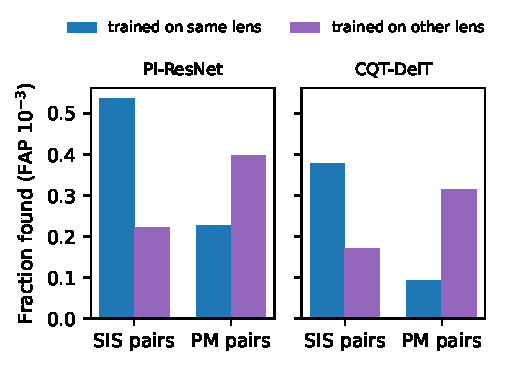
\includegraphics[width=0.95\columnwidth]{figures/fig_transfer.pdf}
\caption{Fraction of lensed pairs recovered at $\pfa=10^{-3}$ when the network is trained on the same lens model as the test pairs (blue) or on the other model (purple).}
\label{fig:transfer}
\end{figure}

\subsection{Computational cost}

On one NVIDIA RTX 5000 Ada GPU, \PIR{} needs $0.73$\,ms per pair for the network and $0.51$\,ms for preparing the input, about $1.2$\,ms in total.
CQT--DeiT needs only $0.22$\,ms for its network, but constructing the two time--frequency images costs $66$\,ms per pair, giving about $66$\,ms in total, roughly fifty times slower.
For a year of Einstein Telescope data with $\sim5\times10^{9}$ pairs, these costs correspond to about $70$ GPU-days and ten GPU-years, respectively.
Even the faster test cannot sensibly be applied to every pair, which motivates the physical pre-selection discussed in Sec.~\ref{sec:catalogue}.

%=====================================================================
\section{What the network does and does not use}
\label{sec:diagnostics}
%=====================================================================

\paragraph*{Time delay.}
Because both segments are aligned on their peaks, the time delay cannot influence the score.
We confirmed this by changing the lens redshift, and hence the delay, in $60$ controlled cases while holding everything else fixed: after peak alignment the inputs to the network (which have unit variance) differed by at most $2.4\times10^{-7}$.
The time delay is nevertheless physically informative---galaxy lenses rarely produce delays longer than a year (Sec.~\ref{sec:delays})---so it must be used outside the network, as we do in Sec.~\ref{sec:catalogue}.

\paragraph*{Type-II phase shift.}
The second image in our simulations is a type-II image, phase-shifted by $\pi/2$ [Eq.~\eqref{eq:image}].
To test whether the network's score responds to this shift, we took $500$ sources from catalogue~B and created, for each, a counterfactual second image without the shift (by undoing the Hilbert transform), keeping the source, magnification and noise realisation identical.
The score changed by $-0.014$ ($-0.046$ to $+0.018$) on average for SIS and by $-0.004$ ($-0.028$ to $+0.021$) for point masses, consistent with zero; the fraction recovered at the frozen $10^{-3}$ threshold also did not change measurably.
This null result is physically reasonable.
For signals dominated by the quadrupole $(\ell,m)=(2,2)$ harmonic, a $\pi/2$ phase shift is almost indistinguishable from a change of the unknown orbital phase at merger~\cite{Ezquiaga2021,Wang2021typeII}; it becomes measurable only through higher harmonics, precession or very high SNR.
The experiment tests the network, not the physics: it shows that the present network does not exploit the Morse phase, not that the phase is absent.

%=====================================================================
\section{The real catalogues: O1--O3, O4a and O4b}
\label{sec:catalogue}
%=====================================================================

We now ask what the numbers of Sec.~\ref{sec:results} imply for the real LIGO--Virgo--KAGRA catalogues.
\PIR{} itself was trained on simulated Einstein Telescope data and cannot be applied to LIGO--Virgo strain without retraining on the corresponding noise (Sec.~\ref{sec:limits}).
What can be done now is to establish, from the published catalogues, how many pairs a pair test would face, how many of them survive simple physical requirements, and therefore which false-alarm probability a pair test must reach.
This follows the logic of recent catalogue-level lensing analyses~\cite{Campailla,Caliskan2023}.

\subsection{Catalogue contents}

We use the binary black holes from O1--O3 with public parameter-estimation results (GWTC-2.1 and GWTC-3~\cite{GWTC21,GWTC3}; network SNR above 9; 63 events: 3 in O1, 7 in O2, 31 in O3a and 22 in O3b) and the binary black holes of O4b from the GWTC-5.0 search release~\cite{GWTC5} (probability of being a binary black hole above $0.5$ and false-alarm rate below one per year; 105 events between 2024 April and 2025 January).
For each event we take the arrival time, the most probable sky position and the area of the $90\%$ sky region, the network SNR, and the detector-frame chirp mass $\mathcal M_{\rm det}=(1+z)\mathcal M$, which governs the frequency evolution and is unchanged by lensing.
For O1--O3 we convert the published source-frame chirp mass to the detector frame using the median redshift; for O4b we use the chirp mass of the best-matching search template, which is less precise.
The O4a catalogue, GWTC-4.0~\cite{GWTC4}, lists about 130 candidates on the Gravitational Wave Open Science Center~\cite{GWOSC_O3}; its sky maps could not be retrieved for this version of the analysis, and the required extraction script is provided with the code so that the numbers below can be updated (Sec.~\ref{sec:o4a}).
The 168 events form $14\,028$ pairs ($1\,953$ within O1--O3 and $5\,460$ within O4b; Table~\ref{tab:funnel}).

\subsection{How long are lensing delays?}
\label{sec:delays}

Figure~\ref{fig:delays} shows the distribution of delays between the two images.
For the priors of our simulation, $97\%$ of SIS delays and all point-mass delays are shorter than a year.
For a more realistic galaxy population---velocity dispersions drawn from the measured distribution of galaxies~\cite{Choi2007} weighted by the lensing cross-section $\propto\sigma_v^4$, lenses distributed in distance according to the lensing probability, source redshifts drawn from the O1--O3 events (median $z_s=0.28$), and $y$ distributed over the full multiple-image region---the median delay is $12$ days.
Detected lensed pairs are additionally biased towards small $y$, because both images must be loud enough to be detected; weighting by the probability that the fainter image is detectable (for the $\rho^{-4}$ distribution of SNRs expected for sources uniform in volume~\cite{Schutz2011}) shortens the median to $2$ days.
In every case more than $99.9\%$ of galaxy-lens delays are shorter than one year, in agreement with previous estimates~\cite{Haris2018,Oguri2018}.
Two physical consequences follow.
First, pairs of events from different observing runs separated by several years, such as O3 and O4b, are very unlikely to be galaxy-lensed pairs (cluster-scale lenses, not considered here, can produce longer delays).
Second, the second image of a lensed event detected near the end of a run may arrive after the run has ended: in our injections (below) $1.5$--$3\%$ of second images fall outside the observing run of the first image, before accounting for detector down time.

\begin{figure}[t]
\centering
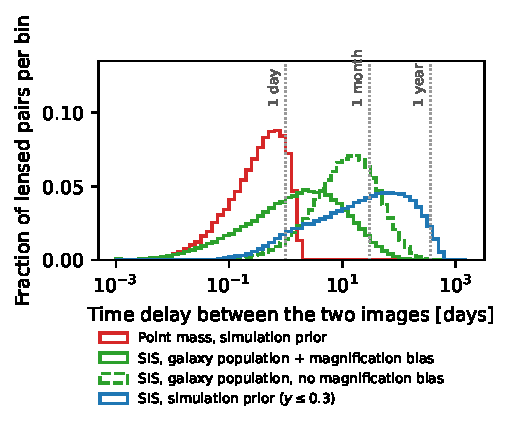
\includegraphics[width=\columnwidth]{figures/fig_time_delays.pdf}
\caption{Time delay between the two images of a strongly lensed binary black hole.
Blue and red: the singular-isothermal-sphere and point-mass priors used to build the simulated catalogues.
Green: singular isothermal spheres drawn from the observed galaxy population, without (dashed) and with (solid) the preference for well-aligned, highly magnified systems among detected pairs.
Dotted lines mark one day, one month and one year.}
\label{fig:delays}
\end{figure}

\subsection{Three physical requirements}

A lensed pair must satisfy three conditions that follow directly from Sec.~\ref{sec:physics}.
We apply them in sequence, each at a level that a genuine pair would pass $99\%$ of the time:
\begin{enumerate}
\item \emph{Allowed delay:} the two events are less than one year apart.
\item \emph{Same sky position:} the angular separation $\theta$ of the two most probable positions is compatible with the two localisation uncertainties.
We approximate each sky region by a circular Gaussian of width $\sigma$ such that its $90\%$ area equals the published value, and require $\chi^2_{\rm sky}=\theta^2/(\sigma_1^2+\sigma_2^2)<9.21$.
\item \emph{Same chirp mass:} the detector-frame chirp masses agree within their uncertainties, $|\ln\mathcal M_{{\rm det},1}-\ln\mathcal M_{{\rm det},2}| < 2.58\,(s_1^2+s_2^2)^{1/2}$, where we adopt fractional uncertainties $s=0.07$ for parameter-estimation values and $s=0.15$ for search-template values.
\end{enumerate}
We do not require consistent luminosity distances or SNRs, because magnification changes both.

\begin{table}[t]
\caption{Number of real event pairs remaining after each physical requirement.
The last column gives the fraction of all pairs that survive.
For comparison, the catalogue-level analysis of Ref.~\cite{Campailla} forwarded $185$ of $3\,655$ GWTC-3 pairs ($5.1\%$) for follow-up.}
\label{tab:funnel}
\begin{ruledtabular}
\begin{tabular}{lrrrrr}
Catalogue & All & $\Delta t<1$\,yr & + sky & + $\mathcal M_{\rm det}$ & Kept \\
\hline
O1--O3 (63 events) & 1\,953 & 1\,402 & 574 & 122 & $6.2\%$ \\
O4b (105 events)   & 5\,460 & 5\,460 & 1\,141 & 515 & $9.4\%$ \\
All (168 events)   & 14\,028 & 6\,862 & 1\,715 & 637 & $4.5\%$ \\
\end{tabular}
\end{ruledtabular}
\end{table}

\begin{figure}[t]
\centering
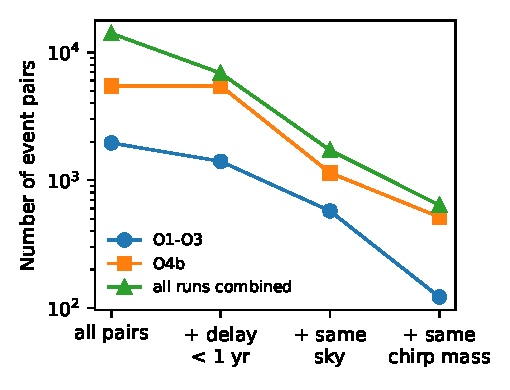
\includegraphics[width=0.95\columnwidth]{figures/fig_catalog_funnel.pdf}
\caption{Number of real event pairs after each physical requirement, for O1--O3, O4b and the combined catalogue (Table~\ref{tab:funnel}).}
\label{fig:funnel}
\end{figure}

Table~\ref{tab:funnel} and Figs.~\ref{fig:funnel} and~\ref{fig:plane} show the result.
The delay requirement removes all pairs that straddle the four-year gap between O3 and O4b, i.e.\ half of the combined catalogue.
The sky requirement is the most powerful single test, removing about three quarters of the remaining pairs, and the chirp-mass requirement removes most of what is left.
Overall $637$ of $14\,028$ pairs ($4.5\%$) survive, a reduction comparable to that of Ref.~\cite{Campailla}.
The number depends on the assumed chirp-mass precision: halving or doubling the tolerance gives $367$ or $1\,010$ surviving pairs.
Requiring delays below $90$ or $30$ days instead of one year leaves $313$ or $116$ pairs; the $30$-day limit, however, would already lose $4$--$24\%$ of genuine galaxy-lensed pairs (Fig.~\ref{fig:delays}).

\begin{figure}[t]
\centering
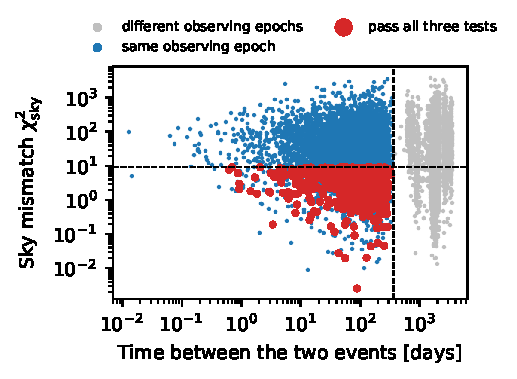
\includegraphics[width=\columnwidth]{figures/fig_real_pairs_plane.pdf}
\caption{All $14\,028$ real event pairs in the plane of time separation and sky mismatch.
Grey: pairs from different observing epochs (O1--O3 versus O4b).
Blue: pairs from the same epoch.
Red: pairs that also pass the chirp-mass requirement.
Dashed lines mark the one-year delay limit and the $99\%$ sky-consistency limit.}
\label{fig:plane}
\end{figure}

\paragraph*{Does the pre-selection keep genuine lensed pairs?}
We injected $4\,000$ synthetic second images for each of O1--O3 and O4b.
Each injection takes a real event as the first image, draws a delay from the galaxy-population distribution of Fig.~\ref{fig:delays}, and gives the second image a localisation uncertainty and a chirp-mass uncertainty drawn from the real catalogue.
Of the injected pairs whose second image falls inside the observing run, $97.8\%$ (O1--O3) and $98.0\%$ (O4b) pass all three requirements.
At the same time, a median of $3$ (O1--O3) and $8$ (O4b) unrelated real events also pass together with the true partner; if the surviving candidates are ordered by their combined mismatch $\chi^2_{\rm sky}+\chi^2_{\mathcal M}$, the true partner is first in $64\%$ and $45\%$ of cases and among the first ten in $97\%$ and $96\%$.
The larger confusion in O4b reflects its higher event density and the lower precision of search-template chirp masses.
We stress that the $99\%$ design pass rate of the sky and chirp-mass requirements holds only if the adopted uncertainty model is correct; the injections test the bookkeeping, not that model.

\paragraph*{A historical candidate.}
The pair GW170104--GW170814, discussed as a possible lensed pair in O2~\cite{Dai2020}, has consistent chirp masses but fails our sky requirement ($\chi^2_{\rm sky}=162$): the most probable positions are $111^\circ$ apart.
GW170104 was observed by two detectors only and its sky region is a long, curved band that a single circular Gaussian represents poorly.
A companion analysis that compares the full sky-position samples of the two events finds them compatible, ranking each event among the top four partners of the other.
This example shows that the circular approximation used here is adequate for counting, but that any pair forwarded for follow-up must be judged with the full sky maps.

\paragraph*{Surviving real pairs.}
The most consistent surviving pairs are listed in Table~\ref{tab:survivors}.
With ${\sim}0.2$ genuine lensed pairs expected in the whole catalogue (next subsection), essentially all of the $637$ survivors must be chance coincidences.
Their agreement in sky position and chirp mass is not evidence for lensing; it is exactly the background that any subsequent test has to reject.
We make no claim that any of these pairs is lensed.

\begin{table}[t]
\caption{The five real pairs with the smallest combined mismatch among the $637$ survivors.
These illustrate the background that a pair test must reject; none is claimed to be lensed.}
\label{tab:survivors}
\footnotesize
\begin{ruledtabular}
\begin{tabular}{lrrr}
Pair & $\Delta t$ [d] & $\theta$ [$^\circ$] & $\mathcal M_{\rm det}$ [$\msun$] \\
\hline
GW240612\_081540 -- GW240908\_082628 & 88.0 & 0.9 & 42.7 / 44.7 \\
GW240420\_175625 -- GW240615\_113620 & 55.7 & 5.7 & 34.9 / 33.4 \\
GW240512\_024139 -- GW240916\_184352 & 127.7 & 1.5 & 10.5 / 9.8 \\
GW240501\_033534 -- GW250108\_152221 & 252.5 & 2.8 & 46.6 / 43.4 \\
GW191222\_033537 -- GW200128\_022011 & 36.9 & 20.5 & 51.0 / 50.0 \\
\end{tabular}
\end{ruledtabular}
\end{table}

\subsection{The false-alarm budget}
\label{sec:budget}

If a pair test with false-alarm probability per pair $\pfa$ is applied to $N_{\rm pair}$ unrelated pairs, the expected number of false acceptances is simply $N_{\rm pair}\,\pfa$.
This must be compared with the expected number of genuine lensed pairs, $N_{\rm lens}\simeq f\,N_{\rm ev}$, where $N_{\rm ev}$ is the number of events and $f\sim10^{-3}$ (plausibly $3\times10^{-4}$--$3\times10^{-3}$) is the fraction of detected binary black holes with a detectable lensed counterpart~\cite{Ng2018,Li2018,Oguri2018,Wierda2021,Xu2022}.
For our 168 events $N_{\rm lens}\approx0.17$ ($0.05$--$0.5$).

Figure~\ref{fig:budget} shows the comparison.
Applied to all $14\,028$ pairs at the primary threshold $\pfa=10^{-3}$, a pair test would accept about $14$ unrelated pairs, nearly a hundred times more than the expected number of genuine ones.
After the physical requirements the expectation drops to $0.64$ at $\pfa=10^{-3}$ and $0.06$ at $\pfa=10^{-4}$.
To keep the expected number of false acceptances below $0.1$---so that a single accepted pair would be meaningful---a pair test applied to the pre-selected pairs needs $\pfa\lesssim1.6\times10^{-4}$, and one applied to all pairs needs $\pfa\lesssim7\times10^{-6}$.
These requirements become more stringent as catalogues grow: adding the roughly 130 O4a candidates of GWTC-4.0 would up to triple the number of pairs, and, unlike O3--O4b pairs, many O4a--O4b pairs are separated by less than a year.
This is the catalogue-level ``look-elsewhere effect'' discussed in Ref.~\cite{Caliskan2023}, expressed in terms of the operating points of a pair test.

\begin{figure}[t]
\centering
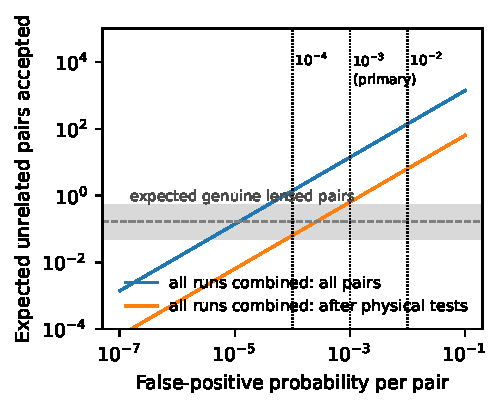
\includegraphics[width=0.95\columnwidth]{figures/fig_false_alarm_budget.pdf}
\caption{Expected number of unrelated real pairs that a pair test would wrongly accept, as a function of its false-alarm probability per pair, for all $14\,028$ pairs of the combined O1--O3 and O4b catalogue (blue) and for the $637$ pairs that pass the physical requirements (orange).
The grey band shows the expected number of genuine lensed pairs, $0.05$--$0.5$.
Vertical lines mark the three operating points calibrated for \PIR{}.}
\label{fig:budget}
\end{figure}

\subsection{Adding O4a}
\label{sec:o4a}

The O4a catalogue can be added without changing the method.
The script \nolinkurl{scripts/gwtc/01c_extract_gwtc4_observables.py} retrieves the GWTC-4.0 search results and sky maps in the same format as GWTC-5.0, and \nolinkurl{05_catalog_context_for_pair_verification.py} then includes O4a automatically, including the O4a--O4b pairs.
We expect the conclusions of this section to be strengthened rather than changed: more pairs require a lower false-alarm probability per pair.

%=====================================================================
\section{Limitations and next steps}
\label{sec:limits}
%=====================================================================

The quantitative results of Secs.~\ref{sec:results} and~\ref{sec:diagnostics} hold for simulated Einstein Telescope data in stationary Gaussian noise.
They do not establish robustness to non-stationary noise, short noise transients (``glitches''), calibration uncertainties or real detector data.
The test compares two pre-selected, peak-aligned segments; it does not detect events, search a catalogue, or replace a Bayesian comparison of the full parameter estimates~\cite{Haris2018,LoHernandez2023,Janquart2021GOLUM}.
The simulated lenses cover only $y\le0.3$ and idealised mass profiles; realistic galaxy lenses with ellipticity and external shear, and lenses that produce more than two images, are not included.
The network does not use the Morse phase or the time delay.
Earlier exploratory results for LIGO-like detectors were obtained with a different evaluation procedure and are not reported here.

Section~\ref{sec:catalogue} suggests a concrete path towards real-data application.
(i) Retrain the network on simulated signals injected into real O4 noise, so that its background is measured in the noise it will face.
(ii) Measure the false-alarm probability per pair to $\lesssim10^{-5}$, which requires of order $10^{6}$--$10^{7}$ unrelated pairs, for example by pairing real events with time-shifted noise.
(iii) Apply it only to pairs that pass the physical pre-selection, which reduces the number of pairs by a factor of about twenty.
(iv) Forward the few accepted pairs to a full Bayesian analysis using the complete sky maps and parameter estimates.
In this chain the pair test contributes speed and an independent, waveform-level view of the data; the physical pre-selection contributes the delay and sky information that the network, by construction, does not use.

%=====================================================================
\section{Conclusions}
\label{sec:conclusions}
%=====================================================================

We have measured the performance of a time-domain pair test for strongly lensed gravitational waves in the way a search is characterised: background fixed in advance from deliberately unrelated pairs, efficiency measured on an independent catalogue.
For simulated Einstein Telescope data, \PIR{} recovers about half of galaxy-lensed and a quarter of point-mass-lensed pairs at a false-alarm probability of $10^{-3}$ per pair, outperforming a time--frequency-image method by about $15$ percentage points and running fifty times faster.
Its performance is governed by the loudness of the fainter image; it ignores, by construction, the time delay and, empirically, the type-II phase shift.
Confronted with the real O1--O3 and O4b catalogues, three physical requirements reduce $14\,028$ pairs to $637$ while keeping $98\%$ of simulated lensed pairs, but a pair test must then reach a false-alarm probability of order $10^{-4}$ or below to make a lensing claim credible, a requirement that will tighten further once O4a and later data are included.
Fast pair tests are therefore most valuable as a calibrated intermediate stage between physical pre-selection and full Bayesian follow-up, and their decisive test will be on real detector noise.

\begin{acknowledgments}
\TBD{Acknowledgements.}
This research has made use of data or software obtained from the Gravitational Wave Open Science Center (gwosc.org), a service of the LIGO Scientific Collaboration, the Virgo Collaboration, and KAGRA.
\end{acknowledgments}

\appendix

%=====================================================================
\section{Plain-language glossary}
\label{app:glossary}
%=====================================================================

\begin{table}[h]
\caption{Terms used in this paper and their meaning.}
\label{tab:glossary}
\begin{ruledtabular}
\begin{tabular}{p{0.32\columnwidth}p{0.6\columnwidth}}
Term & Meaning \\
\hline
Pair score & Number between 0 and 1 returned by the network; high means ``looks like two copies of one signal''. \\
Unrelated pair & Two events known (in simulation) to come from different sources; used to measure the background. \\
False-alarm probability per pair, $\pfa$ & Fraction of unrelated pairs whose score exceeds the threshold. Called ``false-positive probability'' in earlier versions. \\
Detection efficiency, $\eff$ & Fraction of genuine lensed pairs whose score exceeds the threshold. \\
Threshold-setting subset & Part of catalogue~B used only to fix the threshold (analogous to background estimation with time slides). \\
Measurement subset & Part of catalogue~B used only to measure $\eff$; examined only after all choices were frozen (blind analysis). \\
Resampling uncertainty & Spread of a result when the analysis is repeated on randomly re-drawn groups of sources (bootstrap). \\
Selection function & Efficiency as a function of physical properties of the pair (SNR, $y$, magnification ratio). \\
Training & Adjusting the network's internal parameters on catalogue~A to make lensed pairs score high and unrelated pairs low. \\
\end{tabular}
\end{ruledtabular}
\end{table}

%=====================================================================
\section{Network architecture and training}
\label{app:architecture}
%=====================================================================

Each input segment ($1$ channel, \TBD{4\,096} samples) passes through a convolutional stem ($128$ filters, width $15$, stride $2$, max-pooling), three stages of residual blocks with widths $128\to256\to512\to1024$ channels and filter lengths $15$, $11$, $9$, $7$, and global average- and max-pooling, giving a $2048$-dimensional summary per event.
Each residual block contains two convolutions with batch normalisation, the periodic ``Snake'' activation $x+\sin^2(\alpha x)/\alpha$ with learnable $\alpha$~\cite{Snake}, and squeeze-and-excitation channel weighting~\cite{SENet}.
The two summaries $\mathbf u_1,\mathbf u_2$ are combined into $[\mathbf u_1\odot\mathbf u_2,\;|\mathbf u_1-\mathbf u_2|]$ and passed to a two-layer classifier ($256$ hidden units, dropout $0.7$) whose output is converted to the pair score by a logistic function.
Training used the binary cross-entropy loss, the \TBD{optimiser} with learning rate $10^{-4}$ and weight decay $10^{-4}$, batches of $64$ pairs, $300$ epochs, equal numbers of lensed and unrelated pairs drawn afresh in every epoch, and random independent time shifts of up to $1\,024$ samples applied to half of the training pairs.
Catalogue~A was split by source into $2\,000$ training and $500$ validation sources per lens model, and the network from the epoch with the best validation performance was kept (epoch $275$ for SIS, $184$ for point masses).
CQT--DeiT uses a distilled DeiT-tiny transformer~\cite{DeiT} initialised from public image-recognition weights, with the same data, splits and selection rule.

%=====================================================================
\section{Statistical details}
\label{app:stats}
%=====================================================================

\paragraph*{Grouped resampling.}
Sources of catalogue~B are assigned to ten disjoint groups, and unrelated pairs are built only from events in the same group, so that resampling groups never duplicates pairs.
Ninety-five-percent ranges are the $2.5$ and $97.5$ percentiles of $10\,000$ resampled values.
When no unrelated pair of the measurement subset exceeds a threshold, we quote a binomial upper limit rather than zero.

\paragraph*{Summary numbers used in the machine-learning literature.}
The area under the curve of efficiency versus false-alarm probability (AUC) equals the probability that a randomly chosen lensed pair scores higher than a randomly chosen unrelated pair.
On catalogue~B it is $0.989$ (SIS) and $0.985$ (PM) for \PIR{}, and $0.977$ and $0.961$ for CQT--DeiT; the paired differences are $0.012$ ($0.009$--$0.014$) and $0.024$ ($0.021$--$0.027$).
Because the AUC is dominated by easy pairs at high false-alarm probability, it is not a useful figure of merit for a rare-signal search and is not used for any conclusion in the main text.
The classification accuracy at a score threshold of $0.5$ was compared with an exact McNemar test on identical pairs; it is likewise not used in the main text.

\paragraph*{Re-weighting to common SNR and $y$ distributions.}
Point-mass pairs were assigned weights so that their histogram in $(\ln\rho_{\min},\ln\rho_{\max},y)$, with six bins in each SNR dimension and five in $y$, matched that of the SIS pairs over cells populated by both.
Weights were derived on the threshold-setting subset and applied unchanged to the measurement subset.
The effective numbers of pairs after re-weighting are about $1\,160$ (SIS) and $1\,470$ (PM), and the largest weights are $7.4$ and $4.6$.

\paragraph*{Reproducibility.}
Thresholds, network checkpoints, pair lists and analysis code were frozen, with cryptographic checksums, before the measurement subset was examined.
The real-catalogue analysis of Sec.~\ref{sec:catalogue} is reproduced by \nolinkurl{scripts/gwtc/05_catalog_context_for_pair_verification.py} (random seed $20261001$).

\bibliography{refs}

\end{document}
